

\tikzset{every picture/.style={line width=0.75pt}} %set default line width to 0.75pt        

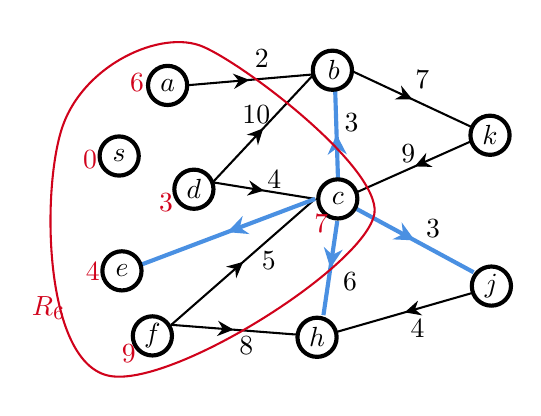
\begin{tikzpicture}[x=0.5pt,y=0.5pt,yscale=-1,xscale=1]
%uncomment if require: \path (0,284); %set diagram left start at 0, and has height of 284

%Straight Lines [id:da3320252336737717] 
\draw [color={rgb, 255:red, 0; green, 0; blue, 0 }  ,draw opacity=1 ][line width=0.75]    (242,47) -- (335,39) ;
\draw [shift={(288.5,43)}, rotate = 535.0799999999999] [fill={rgb, 255:red, 0; green, 0; blue, 0 }  ,fill opacity=1 ][line width=0.08]  [draw opacity=0] (11.61,-5.58) -- (0,0) -- (11.61,5.58) -- (7.71,0) -- cycle    ;
%Straight Lines [id:da02943457575339692] 
\draw [color={rgb, 255:red, 0; green, 0; blue, 0 }  ,draw opacity=1 ][line width=0.75]    (262,117) -- (335,39) ;
\draw [shift={(298.5,78)}, rotate = 493.1] [fill={rgb, 255:red, 0; green, 0; blue, 0 }  ,fill opacity=1 ][line width=0.08]  [draw opacity=0] (11.61,-5.58) -- (0,0) -- (11.61,5.58) -- (7.71,0) -- cycle    ;
%Straight Lines [id:da7032022658079198] 
\draw [color={rgb, 255:red, 0; green, 0; blue, 0 }  ,draw opacity=1 ][line width=0.75]    (262,117) -- (336,129) ;
\draw [shift={(299,123)}, rotate = 189.21] [fill={rgb, 255:red, 0; green, 0; blue, 0 }  ,fill opacity=1 ][line width=0.08]  [draw opacity=0] (11.61,-5.58) -- (0,0) -- (11.61,5.58) -- (7.71,0) -- cycle    ;
%Straight Lines [id:da9416797747261806] 
\draw [color={rgb, 255:red, 0; green, 0; blue, 0 }  ,draw opacity=1 ][line width=0.75]    (232,220) -- (336,129) ;
\draw [shift={(284,174.5)}, rotate = 498.81] [fill={rgb, 255:red, 0; green, 0; blue, 0 }  ,fill opacity=1 ][line width=0.08]  [draw opacity=0] (11.61,-5.58) -- (0,0) -- (11.61,5.58) -- (7.71,0) -- cycle    ;
%Straight Lines [id:da6197316893700862] 
\draw [color={rgb, 255:red, 0; green, 0; blue, 0 }  ,draw opacity=1 ][line width=0.75]    (232,220) -- (322,227) ;
\draw [shift={(277,223.5)}, rotate = 184.45] [fill={rgb, 255:red, 0; green, 0; blue, 0 }  ,fill opacity=1 ][line width=0.08]  [draw opacity=0] (11.61,-5.58) -- (0,0) -- (11.61,5.58) -- (7.71,0) -- cycle    ;
%Straight Lines [id:da7705917014251779] 
\draw [color={rgb, 255:red, 74; green, 144; blue, 226 }  ,draw opacity=1 ][line width=1.5]    (209,177) -- (336,129) ;
\draw [shift={(272.5,153)}, rotate = 339.3] [fill={rgb, 255:red, 74; green, 144; blue, 226 }  ,fill opacity=1 ][line width=0.08]  [draw opacity=0] (14.56,-6.99) -- (0,0) -- (14.56,6.99) -- (9.67,0) -- cycle    ;
%Straight Lines [id:da7178806242260687] 
\draw [color={rgb, 255:red, 0; green, 0; blue, 0 }  ,draw opacity=1 ][line width=0.75]    (449,77) -- (363.5,37) ;
\draw [shift={(406.25,57)}, rotate = 205.07] [fill={rgb, 255:red, 0; green, 0; blue, 0 }  ,fill opacity=1 ][line width=0.08]  [draw opacity=0] (11.61,-5.58) -- (0,0) -- (11.61,5.58) -- (7.71,0) -- cycle    ;
%Straight Lines [id:da2873203830948724] 
\draw [color={rgb, 255:red, 0; green, 0; blue, 0 }  ,draw opacity=1 ][line width=0.75]    (449.5,87) -- (366.5,124) ;
\draw [shift={(408,105.5)}, rotate = 335.97] [fill={rgb, 255:red, 0; green, 0; blue, 0 }  ,fill opacity=1 ][line width=0.08]  [draw opacity=0] (11.61,-5.58) -- (0,0) -- (11.61,5.58) -- (7.71,0) -- cycle    ;
%Straight Lines [id:da9325647569597147] 
\draw [color={rgb, 255:red, 74; green, 144; blue, 226 }  ,draw opacity=1 ][line width=1.5]    (450.5,182) -- (365.5,136) ;
\draw [shift={(408,159)}, rotate = 208.42] [fill={rgb, 255:red, 74; green, 144; blue, 226 }  ,fill opacity=1 ][line width=0.08]  [draw opacity=0] (14.56,-6.99) -- (0,0) -- (14.56,6.99) -- (9.67,0) -- cycle    ;
%Straight Lines [id:da8240281406202591] 
\draw [color={rgb, 255:red, 74; green, 144; blue, 226 }  ,draw opacity=1 ][line width=1.5]    (342,213) -- (352,145) ;
\draw [shift={(347,179)}, rotate = 278.37] [fill={rgb, 255:red, 74; green, 144; blue, 226 }  ,fill opacity=1 ][line width=0.08]  [draw opacity=0] (14.56,-6.99) -- (0,0) -- (14.56,6.99) -- (9.67,0) -- cycle    ;
%Straight Lines [id:da6386544223700206] 
\draw [color={rgb, 255:red, 0; green, 0; blue, 0 }  ,draw opacity=1 ][line width=0.75]    (352,225) -- (449.5,197) ;
\draw [shift={(400.75,211)}, rotate = 343.98] [fill={rgb, 255:red, 0; green, 0; blue, 0 }  ,fill opacity=1 ][line width=0.08]  [draw opacity=0] (11.61,-5.58) -- (0,0) -- (11.61,5.58) -- (7.71,0) -- cycle    ;
%Straight Lines [id:da7268529078901531] 
\draw [color={rgb, 255:red, 74; green, 144; blue, 226 }  ,draw opacity=1 ][line width=1.5]    (352.5,114) -- (350.5,51) ;
\draw [shift={(351.5,82.5)}, rotate = 448.18] [fill={rgb, 255:red, 74; green, 144; blue, 226 }  ,fill opacity=1 ][line width=0.08]  [draw opacity=0] (14.56,-6.99) -- (0,0) -- (14.56,6.99) -- (9.67,0) -- cycle    ;
%Shape: Polygon Curved [id:ds3197703892135201] 
\draw  [color={rgb, 255:red, 208; green, 2; blue, 27 }  ,draw opacity=1 ] (153,78) .. controls (168,32) and (225,6) .. (255,19) .. controls (285,32) and (376,101) .. (379,136) .. controls (382,171) and (236,265) .. (188,257) .. controls (140,249) and (138,124) .. (153,78) -- cycle ;

% Text Node
\draw (129,197) node [anchor=north west][inner sep=0.75pt]   [align=left] {$\displaystyle \textcolor[rgb]{0.82,0.01,0.11}{R}\textcolor[rgb]{0.82,0.01,0.11}{_{6}}$};
% Text Node
\draw (166,92) node [anchor=north west][inner sep=0.75pt]   [align=left] {$\displaystyle \textcolor[rgb]{0.82,0.01,0.11}{0}$};
% Text Node
\draw (290.24,19.06) node [anchor=north west][inner sep=0.75pt]   [align=left] {$\displaystyle 2$};
% Text Node
\draw  [line width=1.5]   (194.38, 98) circle [x radius= 14.15, y radius= 14.15]   ;
\draw (194.38,98) node   [align=left] {$\displaystyle s$};
% Text Node
\draw (200,36) node [anchor=north west][inner sep=0.75pt]   [align=left] {$\displaystyle \textcolor[rgb]{0.82,0.01,0.11}{6}$};
% Text Node
\draw  [line width=1.5]   (229.38, 47) circle [x radius= 14.15, y radius= 14.15]   ;
\draw (229.38,47) node   [align=left] {$\displaystyle a$};
% Text Node
\draw (221,123) node [anchor=north west][inner sep=0.75pt]   [align=left] {$\displaystyle \textcolor[rgb]{0.82,0.01,0.11}{3}$};
% Text Node
\draw  [line width=1.5]   (248.38, 122) circle [x radius= 14.15, y radius= 14.15]   ;
\draw (248.38,122) node   [align=left] {$\displaystyle d$};
% Text Node
\draw (168,173) node [anchor=north west][inner sep=0.75pt]   [align=left] {\textcolor[rgb]{0.82,0.01,0.11}{$\displaystyle 4$}};
% Text Node
\draw  [line width=1.5]   (196.38, 181) circle [x radius= 14.15, y radius= 14.15]   ;
\draw (196.38,181) node   [align=left] {$\displaystyle e$};
% Text Node
\draw  [line width=1.5]   (348.48, 36) circle [x radius= 14.15, y radius= 14.15]   ;
\draw (342.98,36) node [anchor=west] [inner sep=0.75pt]   [align=left] {$\displaystyle b$};
% Text Node
\draw  [line width=1.5]   (352.38, 129) circle [x radius= 14.15, y radius= 14.15]   ;
\draw (352.38,129) node   [align=left] {$\displaystyle c$};
% Text Node
\draw  [line width=1.5]   (462.38, 83) circle [x radius= 14.15, y radius= 14.15]   ;
\draw (462.38,83) node   [align=left] {$\displaystyle k$};
% Text Node
\draw  [line width=1.5]   (337.38, 229) circle [x radius= 14.15, y radius= 14.15]   ;
\draw (337.38,229) node   [align=left] {$\displaystyle h$};
% Text Node
\draw (194,232) node [anchor=north west][inner sep=0.75pt]   [align=left] {$\displaystyle \textcolor[rgb]{0.82,0.01,0.11}{9}$};
% Text Node
\draw  [line width=1.5]   (218.38, 228) circle [x radius= 14.15, y radius= 14.15]   ;
\draw (218.38,228) node   [align=left] {$\displaystyle f$};
% Text Node
\draw  [line width=1.5]   (463.38, 192) circle [x radius= 14.15, y radius= 14.15]   ;
\draw (463.38,192) node   [align=left] {$\displaystyle j$};
% Text Node
\draw (281.24,59.06) node [anchor=north west][inner sep=0.75pt]   [align=left] {$\displaystyle 10$};
% Text Node
\draw (299.24,106.06) node [anchor=north west][inner sep=0.75pt]   [align=left] {$\displaystyle 4$};
% Text Node
\draw (295.24,165.06) node [anchor=north west][inner sep=0.75pt]   [align=left] {$\displaystyle 5$};
% Text Node
\draw (279,226.5) node [anchor=north west][inner sep=0.75pt]   [align=left] {$\displaystyle 8$};
% Text Node
\draw (406.24,34.06) node [anchor=north west][inner sep=0.75pt]   [align=left] {$\displaystyle 7$};
% Text Node
\draw (414,142) node [anchor=north west][inner sep=0.75pt]   [align=left] {$\displaystyle 3$};
% Text Node
\draw (402.75,214) node [anchor=north west][inner sep=0.75pt]   [align=left] {$\displaystyle 4$};
% Text Node
\draw (396,87.47) node [anchor=north west][inner sep=0.75pt]   [align=left] {$\displaystyle 9$};
% Text Node
\draw (355,65) node [anchor=north west][inner sep=0.75pt]   [align=left] {$\displaystyle 3$};
% Text Node
\draw (354,180) node [anchor=north west][inner sep=0.75pt]   [align=left] {$\displaystyle 6$};
% Text Node
\draw (333.24,138.06) node [anchor=north west][inner sep=0.75pt]   [align=left] {$\displaystyle \textcolor[rgb]{0.82,0.01,0.11}{7}$};


\end{tikzpicture}

